\documentclass{article}

\usepackage[preprint]{../mix_n8/neurips_2025}
\usepackage[utf8]{inputenc}
\usepackage[T1]{fontenc}
\usepackage{booktabs}
\usepackage{amsmath}
\usepackage{graphicx}
\usepackage{microtype}
\usepackage{hyperref}
\usepackage{xcolor}

\title{What Fails in Mixed-Orientation GradMem?\\
Token-Level Errors, Controlled Values, and WRITE--READ Misalignment}

\author{Anonymous Author(s)}

\newcommand{\dataset}{\textsc{mix-N8}}
\newcommand{\gm}{GradMem}

\begin{document}
\maketitle

\begin{abstract}
Earlier \dataset{} experiments appeared to show that reconstruction-based \gm{} could not learn mixed forward and backward key--value retrieval.  New runs with step-alignment and intermediate-READ losses disprove that absolute claim: two of three runs exceed 96\% validation exact match (EM).  We analyze all 12 available reconstruction \gm{} runs across five hyperparameter configurations.  On 512 frozen validation examples, unsuccessful 256-dimensional runs are essentially perfect on forward contexts but obtain only 11.7--14.9\% backward EM.  Their backward errors are dominated by a wrong first value token paired with a correct teacher-forced second token.  We introduce a controlled condition that leaves all keys and queries unchanged, makes every value begin with the queried value's first token, and gives the eight values unique second tokens.  This makes the first token uninformative for selecting a pair.  The two successful auxiliary-loss runs retain 94.3\% forward EM but fall to 38.7\% backward EM, with substantial seed variation (48.8\% versus 28.6\%).  Across frozen WRITE trajectories, value reconstruction cross-entropy falls sharply while key cross-entropy remains almost unchanged even in successful models.  Thus the auxiliary losses enable high ordinary-task accuracy without making token reconstruction itself direction-neutral, and ordinary EM conceals substantial backward association fragility.
\end{abstract}

\section{Question and Scope}

\gm{} writes a context into per-example prefix memory by applying gradient descent to autoregressive context reconstruction.  In \dataset{}, forward contexts serialize pairs as \texttt{KK:VV}, backward contexts as \texttt{VV:KK}, and every query requests \texttt{VV} from \texttt{KK}.  Autoregressive reconstruction is directly aligned with the query direction only in forward contexts.

The original experiments found a stable aggregate plateau near 56\% EM: nearly perfect forward retrieval and poor backward retrieval.  Subsequent runs added two outer-loop losses.  Step alignment minimizes one minus the cosine between each reconstruction WRITE gradient and a stopped target-READ gradient at the resulting memory.  Intermediate READ directly supervises the memory after the first of two WRITE steps.  Both losses have weight 0.1 and use query targets only during meta-training; inference-time WRITE remains context-only.  Two of three runs using both losses entered a high-accuracy regime.

This report asks three narrower questions:
\begin{enumerate}
  \item Which of the four two-token correctness patterns dominate each configuration and orientation?
  \item Does high ordinary-task EM imply that the model retrieves the distinguishing second value token when every value shares its first token?
  \item How do alignment, reconstruction, key/value reconstruction, and READ losses relate during training and along frozen WRITE trajectories?
\end{enumerate}

The analysis includes reconstruction \gm{} only.  It does not compare learned-energy objectives.

\section{Evaluation Design}

\subsection{Runs and outcome groups}

We discover every run under \texttt{runs/mix-N8-K2V2-V62\_1M} whose directory begins with \texttt{gradmem}.  This yields 12 runs and five hyperparameter configurations: a 128-dimensional $K=1$ write-head configuration; two 256-dimensional $K=2$ baselines with the base LM head or a separate write head; three write-head runs with step alignment and intermediate READ; and three descendants adding a Lipschitz penalty.  Unless noted, the 256-dimensional runs use eight memory tokens, inner SGD learning rate 0.4, full second-order differentiation, batch size 64, and outer learning rate $10^{-4}$.

A run is called successful when its best recorded full-validation EM is at least 90\%.  This threshold separates the two 96--99\% runs from the directional plateau and the partially improved 73.2\% Lipschitz run.  ``Unsuccessful'' is descriptive, not a statement of eventual impossibility: several recent runs were still active when the manifest was generated.  Frozen evaluation uses each Trainer-selected best-token-accuracy checkpoint.

\subsection{Controlled shared-first-value contexts}

For each of the first 512 validation examples (264 forward, 248 backward), we construct a paired controlled example.  All keys, the query, context orientation, syntax, pair positions, and non-pair context characters are unchanged.  The queried value is unchanged.  Every distractor value is changed to begin with the queried value's first character, and all eight second characters are made unique.  Consequently, the first target token identifies no pair; correct second-token prediction requires selecting the queried association among eight values.  The transformation is deterministic and identical for every checkpoint.

\subsection{Teacher-forced error taxonomy}

READ evaluation follows the training evaluator and scores target logits under teacher forcing.  In particular, the second-token prediction is conditioned on the gold first target token even when the model predicts the first token incorrectly.  We therefore report the mutually exclusive patterns
\begin{align*}
  &\text{both correct}, &&\text{first correct / second wrong},\\
  &\text{first wrong / second correct}, &&\text{both wrong}.
\end{align*}
The ``second-only'' category must not be interpreted as free-running exact generation.  For wrong second-token predictions, we additionally record whether the prediction equals a distractor value's second token.

\subsection{Loss diagnostics}

We replay every frozen WRITE trajectory through $M_K$.  At each state we measure per-example total reconstruction CE, semantic key CE, semantic value CE, target READ loss, memory-gradient norm, and the cosine between the incoming WRITE gradient and target-READ gradient.  The final per-example alignment loss averages the transition cosines and the final reconstruction-gradient cosine using the same unnormalized cosine convention as training.

Training-history correlations use every recorded full-validation point in \texttt{trainer\_state.json}.  We report within-run Spearman correlation.  These histories are highly nonstationary and autocorrelated; the correlations are descriptive and are not effective-sample-size-adjusted significance tests.

\section{Results}

\subsection{Ordinary performance is dominated by orientation}

Figure~\ref{fig:condition-em} shows frozen-checkpoint EM for every run.  All 256-dimensional configurations are nearly perfect on clean forward examples.  Without the new losses, clean backward EM remains between 11.7\% and 14.9\%.  The auxiliary-loss configuration changes this outcome in two seeds: their clean backward EM is 98.0\% and 95.6\%, while seed 144 remains at 13.3\%.  The Lipschitz runs do not cross the 90\% run-level success threshold; seed 143 partially improves to 45.2\% backward EM at its selected checkpoint.

\begin{figure}[t]
  \centering
  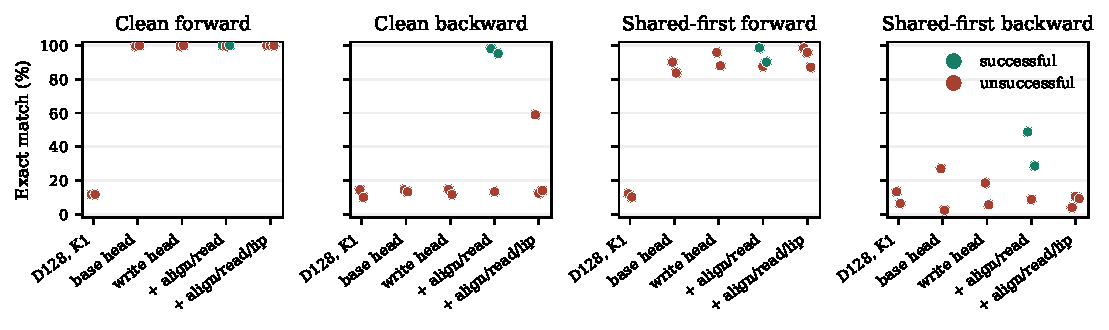
\includegraphics[width=\linewidth]{figures/condition_exact_match.pdf}
  \caption{Frozen exact match for all 12 runs on 512 paired examples.  Each point is one run; green and red denote success or failure under the 90\% full-validation threshold.  The shared-first-value condition preserves keys and targets but makes all values share the target's first token and gives them unique second tokens.}
  \label{fig:condition-em}
\end{figure}

\begin{table}[t]
  \caption{Pooled frozen-checkpoint EM by hyperparameter and outcome group.  Values are percentages over run--example evaluations and therefore describe the observed runs rather than independent confidence intervals.}
  \label{tab:summary}
  \centering
  \small
  \begin{tabular}{llrrrr}
    \toprule
    Configuration & Outcome & Clean F & Clean B & Shared-first F & Shared-first B \\
    \midrule
    D128, $K=1$ & unsuccessful & 11.7 & 12.3 & 11.2 & 9.9 \\
    Base head & unsuccessful & 99.8 & 13.9 & 86.9 & 14.7 \\
    Write head & unsuccessful & 99.8 & 13.3 & 91.9 & 12.1 \\
    + alignment/READ & successful & 100.0 & 96.6 & 94.3 & 38.7 \\
    + alignment/READ & unsuccessful & 99.6 & 13.3 & 87.5 & 8.9 \\
    + alignment/READ/Lipschitz & unsuccessful & 100.0 & 28.5 & 93.8 & 7.9 \\
    \bottomrule
  \end{tabular}
\end{table}

\subsection{The controlled condition exposes second-token association failure}

The shared-first-value manipulation leaves forward retrieval comparatively strong but sharply reduces backward retrieval.  Among successful auxiliary-loss runs, pooled forward EM falls modestly from 100.0\% to 94.3\%, whereas backward EM falls from 96.6\% to 38.7\%.  The two successful seeds differ substantially: seed 143 obtains 48.8\% and seed 145 obtains 28.6\% controlled backward EM.  Thus high ordinary backward EM does not imply robust selection of the distinguishing second value token.

The failed 256-dimensional models show the same phenomenon more strongly.  In clean backward contexts, their first-token accuracy is only approximately 16--19\%, while teacher-forced second-token accuracy is 94--97\%.  Once all first value tokens are made identical, first-token accuracy becomes nearly trivial but backward second-token accuracy is only 2--27\% depending on seed.  Most wrong second tokens are copied from distractor values: the run-level rate reaches 73--98\% of all controlled backward examples in the base-head and write-head baselines.

Figure~\ref{fig:taxonomy} makes the mode switch explicit.  Clean backward failures are dominated by ``second only.''  Controlled backward failures become predominantly ``first only'': the common first token is recovered, but the model selects the wrong second token.  The manipulation therefore converts an ambiguous ordinary metric pattern into a direct test of pair-specific association.

\begin{figure}[t]
  \centering
  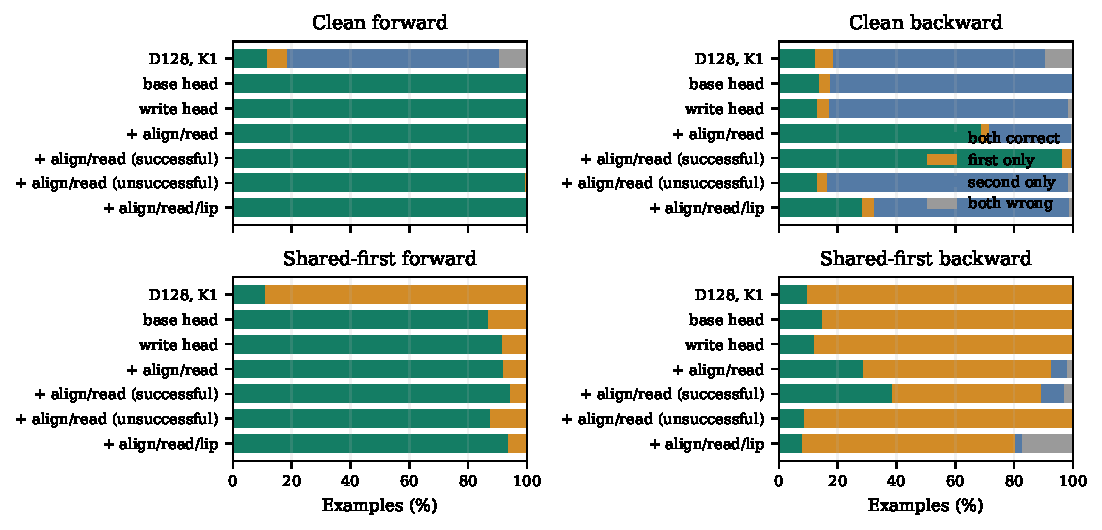
\includegraphics[width=\linewidth]{figures/failure_taxonomy.pdf}
  \caption{Teacher-forced two-token correctness taxonomy, pooled within hyperparameter and outcome groups.  ``Second only'' means that the second token is correct when conditioned on the gold first token.  The controlled backward condition is dominated by a correct common first token and an incorrect distinguishing second token.}
  \label{fig:taxonomy}
\end{figure}

\subsection{Successful WRITE still reconstructs values, not keys}

Table~\ref{tab:trajectory} and Figure~\ref{fig:trajectory} show that the new losses do not qualitatively change which semantic tokens reconstruction optimizes.  In every 256-dimensional group, value CE falls from roughly 4.3--4.6 to 0.9--1.2.  Key CE changes little.  In the successful auxiliary runs it slightly increases, from 4.85 to 4.86, while READ loss falls from 3.13 to 0.009.

\begin{table}[t]
  \caption{Mean clean-context frozen trajectory from $M_0$ to $M_K$.  Successful and unsuccessful members of the joint auxiliary-loss configuration are split.}
  \label{tab:trajectory}
  \centering
  \small
  \begin{tabular}{llrrr}
    \toprule
    Configuration & Outcome & Key CE & Value CE & READ loss \\
    \midrule
    D128, K1 & unsuccessful & 4.33$\to$4.33 & 4.21$\to$3.48 & 2.36$\to$1.668 \\
base head & unsuccessful & 4.39$\to$4.22 & 4.33$\to$1.01 & 3.88$\to$0.265 \\
write head & unsuccessful & 4.35$\to$4.31 & 4.34$\to$0.93 & 3.17$\to$0.265 \\
+ align/read & successful & 4.85$\to$4.86 & 4.58$\to$1.15 & 3.13$\to$0.009 \\
+ align/read & unsuccessful & 4.26$\to$4.25 & 4.33$\to$1.06 & 2.38$\to$0.269 \\
+ align/read/lip & unsuccessful & 4.37$\to$4.34 & 4.44$\to$1.01 & 4.33$\to$0.225 \\

    \bottomrule
  \end{tabular}
\end{table}

\begin{figure}[t]
  \centering
  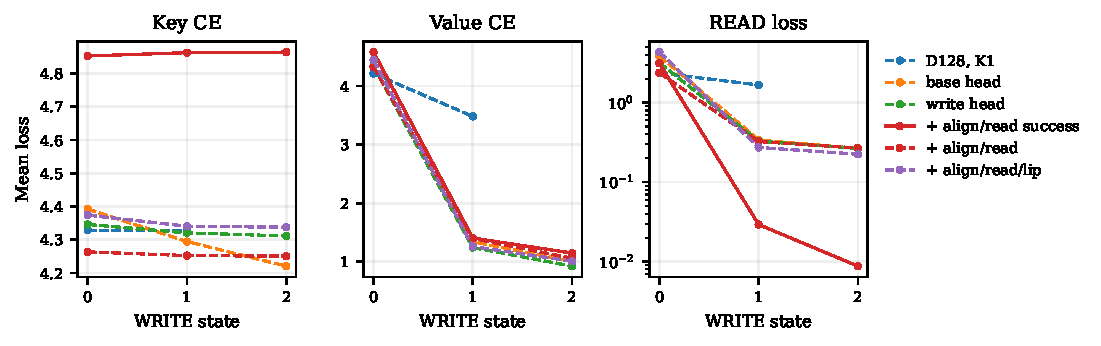
\includegraphics[width=0.94\linewidth]{figures/loss_trajectories.pdf}
  \caption{Mean semantic reconstruction and target READ losses along clean frozen trajectories.  Solid lines denote the successful auxiliary-loss group; dashed lines denote unsuccessful groups.  Key CE remains nearly flat even when READ loss approaches zero.}
  \label{fig:trajectory}
\end{figure}

This revises the causal interpretation of the earlier diagnostic.  Flat key reconstruction accompanies failure, but it is not sufficient to explain failure: it also accompanies successful retrieval.  The relevant information can be carried by reconstruction gradients without making the context keys predictable under the write head.  Step alignment and intermediate READ appear to change how the outer loop uses the trajectory rather than making autoregressive reconstruction symmetric.

\subsection{Alignment tracks READ utility more consistently than reconstruction level}

Across training, worse step alignment (larger one-minus-cosine loss) generally coincides with larger READ loss in the 256-dimensional runs.  Within-run Spearman correlations are 0.806--0.890 for write-head baselines, 0.581--0.893 for the joint auxiliary-loss runs, and 0.620--0.697 with the additional Lipschitz penalty.  The diagnostic therefore tracks READ quality even when its optimization weight is zero.

By contrast, aggregate inner reconstruction loss is not a monotonic proxy for READ utility across outer training.  Its within-run correlation with READ loss ranges from $-0.485$ to 0.239 in write-head baselines and from $-0.569$ to $-0.260$ in successful auxiliary-loss runs.  In those successful runs, READ improves while the overall reconstruction scale can move in the opposite direction.  Figure~\ref{fig:training-correlations} reports every run rather than only group averages.

\begin{figure}[t]
  \centering
  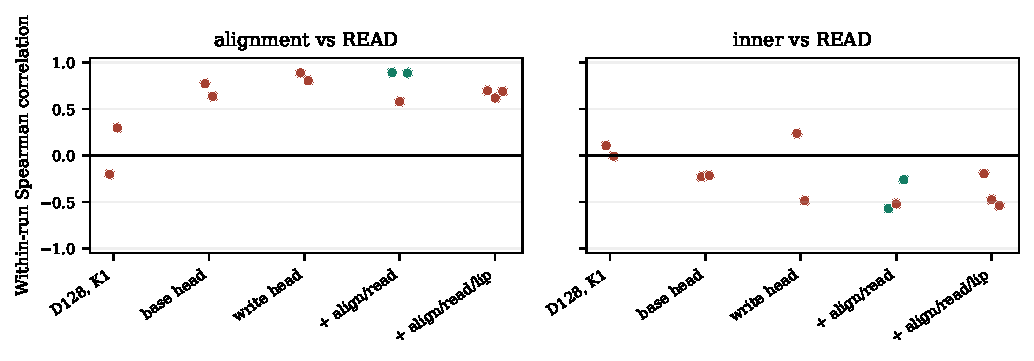
\includegraphics[width=0.9\linewidth]{figures/training_loss_correlations.pdf}
  \caption{Within-run Spearman correlations over full-validation training checkpoints.  Positive alignment--READ correlation means worse cosine alignment accompanies larger READ loss.  Correlations are descriptive over autocorrelated trajectories.}
  \label{fig:training-correlations}
\end{figure}

The frozen per-example analysis is compatible with this distinction.  Within the aligned configuration, step-alignment loss has Spearman correlation 0.641 with final READ loss in successful runs and 0.636 in the unsuccessful run.  For successful runs, changes in semantic key and value CE correlate 0.666 and 0.683 with final READ loss, respectively, while total inner-loss change has correlation $-0.021$.  Total context reconstruction includes syntax and filler tokens, so cancellation and token-count weighting can obscure the role-specific relationships.

These correlations do not identify the treatment effect of the alignment loss.  The unweighted baselines already log the same diagnostic, and alignment and intermediate READ were enabled together.  A factorial ablation is required to separate their effects.

\section{Interpretation}

\paragraph{What the new losses fix.}
The joint losses can move a run out of the forward-only basin.  Under the matched write-head seed 143 comparison, the no-auxiliary run reaches 56.7\% best full-validation EM, while the auxiliary run reaches 99.0\%.  The successful frozen models solve both clean orientations, and their READ loss is already very low after the first WRITE step.  This is evidence that stronger trajectory-level credit assignment can make reconstruction WRITE useful for inverse retrieval.

\paragraph{What they do not fix.}
They do not make context reconstruction direction-neutral.  Key CE remains flat, and performance remains sensitive to a controlled change that removes first-token value diversity.  Even among successful runs, backward controlled performance is both low and seed-sensitive.  The observed success is therefore narrower than robust recovery of arbitrary two-token associations.

\paragraph{A plausible mechanism.}
The reconstruction gradient is a high-dimensional signal.  Its scalar CE can be dominated by easy value prediction, while task-relevant variation in its direction still carries key-conditioned information.  The alignment loss can reward this useful directional component without requiring key CE itself to decrease.  Intermediate READ supplies direct supervision at $M_1$, shortening the credit path.  This account is consistent with the data but not isolated experimentally because both losses were changed together.

\section{Limitations and Next Tests}

The frozen subset contains 512 deterministic examples rather than all 5,000 validation examples.  Pooled percentages treat run--example evaluations descriptively; training seeds, not examples, are the unit for method-level reliability, and each group has only two or three runs.  Checkpoints are selected by validation token accuracy, so the analysis is selection-conditioned.  Several recent runs were active, making failure labels right-censored.  Teacher forcing makes the four-way token taxonomy diagnostic rather than equivalent to free-running sequence generation.  The controlled contexts are out of distribution and intentionally change value collisions; they measure reliance on first-token diversity, not ordinary validation accuracy.

The immediate decisive experiment is a matched factorial sweep with reconstruction WRITE under: no auxiliary loss, step alignment only, intermediate READ only, and both.  At least five seeds should be run to a common budget, with success probability and time to 90\% EM as primary endpoints.  The shared-first-value evaluation should be included during training only as a held-out diagnostic.  A stronger follow-up would vary the number of distinct first-token groups from one to eight, producing a graded test rather than one clean/OOD contrast.

\section{Conclusion}

Reconstruction \gm{} is not intrinsically unable to solve \dataset{}: two joint auxiliary-loss runs reach high clean accuracy in both orientations.  The older failures nevertheless expose a genuine and highly structured weakness.  They are perfect on forward contexts, predict the first backward value token poorly, and often predict the teacher-forced second token correctly.  Making every value share the first token reveals that both failed and successful models often cannot select the distinguishing backward second token.  Step alignment and intermediate READ improve acquisition of a useful WRITE trajectory, but successful trajectories still sharply reduce value CE while leaving key CE flat.  The main finding is therefore about trajectory-level credit assignment, not the elimination of autoregressive directional bias.

\appendix
\section{Per-Run Results}

Table~\ref{tab:runs} lists the exact frozen subset metrics.  ``Best EM'' is from full-validation training history; the remaining columns are from the fixed 512-example analysis.

\begin{table}[h]
  \caption{All analyzed runs.  Values are percentages.}
  \label{tab:runs}
  \centering
  \scriptsize
  \begin{tabular}{lrlrrrrr}
    \toprule
    Configuration & Seed & Outcome & Best EM & Clean F & Clean B & Shared F & Shared B \\
    \midrule
    D128, K1 & 143 & unsuccessful & 11.1 & 11.7 & 14.5 & 12.1 & 13.3 \\
D128, K1 & 144 & unsuccessful & 12.4 & 11.7 & 10.1 & 10.2 & 6.5 \\
base head & 143 & unsuccessful & 56.5 & 99.6 & 14.5 & 90.2 & 27.0 \\
base head & 144 & unsuccessful & 56.3 & 100.0 & 13.3 & 83.7 & 2.4 \\
write head & 143 & unsuccessful & 56.7 & 99.6 & 14.9 & 95.8 & 18.5 \\
write head & 144 & unsuccessful & 56.6 & 100.0 & 11.7 & 87.9 & 5.6 \\
+ align/read & 143 & successful & 99.0 & 100.0 & 98.0 & 98.5 & 48.8 \\
+ align/read & 144 & unsuccessful & 56.8 & 99.6 & 13.3 & 87.5 & 8.9 \\
+ align/read & 145 & successful & 96.9 & 100.0 & 95.2 & 90.2 & 28.6 \\
+ align/read/lip & 143 & unsuccessful & 76.7 & 100.0 & 58.9 & 98.5 & 4.0 \\
+ align/read/lip & 144 & unsuccessful & 56.7 & 100.0 & 12.5 & 95.8 & 10.5 \\
+ align/read/lip & 145 & unsuccessful & 56.5 & 100.0 & 14.1 & 87.1 & 9.3 \\

    \bottomrule
  \end{tabular}
\end{table}

\section{Reproducibility}

The analysis manifest, raw per-example predictions, trajectories, controlled contexts, grouped summaries, and correlation tables are stored under \texttt{reports/gradmem\_mix\_failures/data}.  The principal files are:
\begin{itemize}
  \item \texttt{checkpoints.csv}: run configuration, outcome, and selected checkpoint;
  \item \texttt{controlled\_contexts.jsonl}: clean and deterministically transformed example pairs;
  \item \texttt{per\_example\_predictions.csv}: raw two-token predictions and taxonomy;
  \item \texttt{trajectory\_losses.csv}: per-state total, key, value, READ, gradient, and cosine diagnostics;
  \item \texttt{training\_history.csv} and \texttt{training\_correlations.csv};
  \item \texttt{frozen\_correlations.csv}, \texttt{failure\_taxonomy.csv}, and \texttt{token\_summary.csv}.
\end{itemize}
The exact commands are recorded in the adjacent \texttt{README.md}.  Frozen models are loaded in float32 and evaluated sequentially on one GPU.  WRITE remains differentiable with respect to fast memory while model parameters are frozen.

\end{document}
